\section{Dynamic systems}
\subsection{}

\begin{frame}\mccz
\frametitleTC{Foreword}
\framesubtitleTC{on how we shall proceed given the breadth of the subject}
\myPause
 \begin{columns}
  \column[T]{0.35\textwidth}
   \only<2 | handout:0>{\centering
\includegraphics[height=6cm]{./Unit-01/img/DynSys-Variety-1_cc0.jpg}}%
   \only<3 | handout:0>{\centering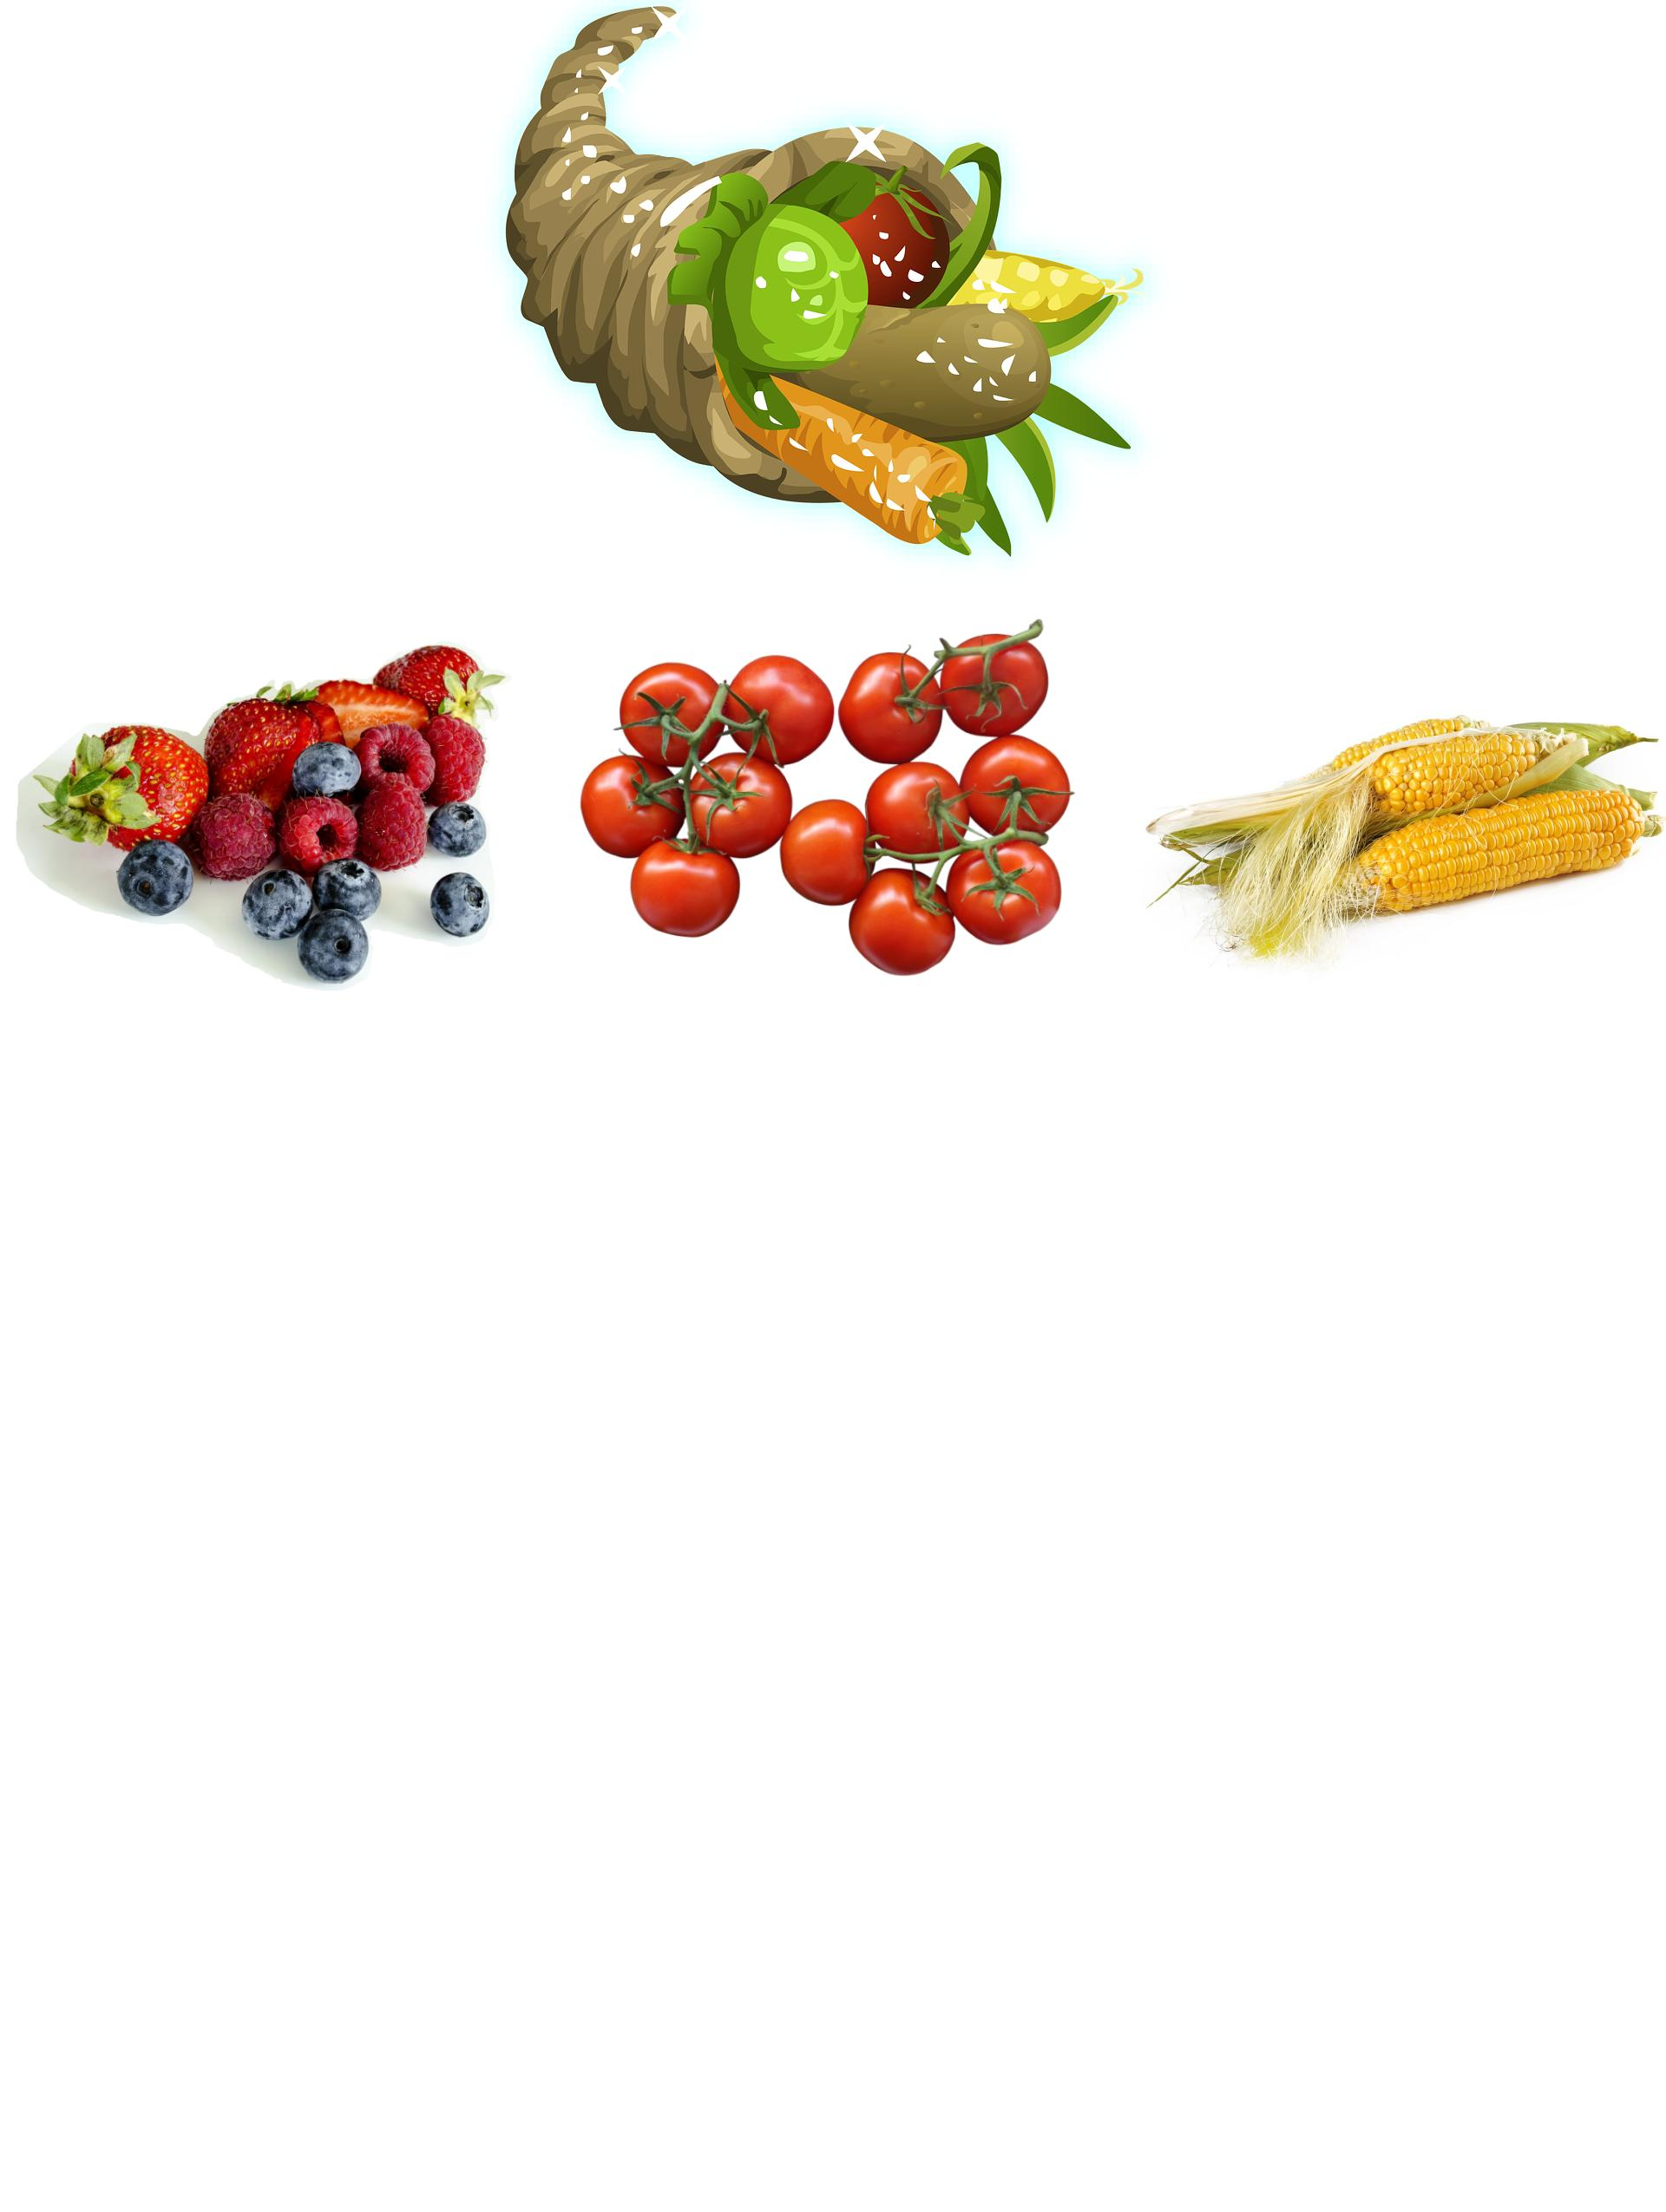
\includegraphics[height=6cm]{./Unit-01/img/DynSys-Variety-2_cc0.jpg}}%
   \only<4 | handout:0>{\centering
\includegraphics[height=6cm]{./Unit-01/img/DynSys-Variety-3_cc0.jpg}}%
   \only<5-           >{\centering
\includegraphics[height=6cm]{./Unit-01/img/DynSys-Variety-4_cc0.jpg}}%
  \column[T]{0.65\textwidth}
   \begin{itemize}[<+-| alert@+>]
   \item We shall state the \underline{general idea} of dynamic system,
   \item \vspace{8mm}then specialise to a few types of interest,
   \item \vspace{8mm}then see what control problems they fit,
   \item \vspace{8mm}and finally restrict to one type\\
         for the purpose of our activity.
   \end{itemize}
 \end{columns}
\end{frame}

\begin{frame}
\frametitleTC{Dynamic system}
\framesubtitleTC{General definition}
\myPause
 \begin{center}
  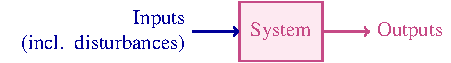
\includegraphics[width=0.6\columnwidth]{./Unit-01/img/DynSys-GenericSystem.pdf}
  \myPause
 \end{center}
 \begin{itemize}[<+-| alert@+>]
 \item Suppose you know the values that the inputs have NOW.
 \item Can you tell which is NOW the values of the outputs?
 \item \vfill If so, the system is \TC{non dynamic}, otherwise it is \TC{dynamic.}
 \item Let us see some examples.
 \end{itemize}
\end{frame}

\begin{frame}
\frametitleTC{Dynamic system}
\framesubtitleTC{Introductory examples (1/3)}
\myPause
 \begin{itemize}[<+-| alert@+>]
 \item \textbf{Example 1}
       \begin{itemize}[<+-| alert@+>]
       \item[] \begin{tabular}{lll}
                System  &: & resistor of resistance $R$.\\
                Input   &: & applied voltage $V(t)$.\\
                Output  &: & flowing current $I(t)$.
               \end{tabular}
       \item \vspace{1mm}At time $\overline{t}$ the input is $V(\overline{t})=\overline{V}$; can you tell what
             the output $I(\overline{t})$ is?
       \item Yes, we have $I(\overline{t})=\overline{V}/R$.
       \item[] $\Rightarrow$ This system is non dynamic. 
       \end{itemize}
 \item \vfill\textbf{Example 2}
       \begin{itemize}[<+-| alert@+>]
       \item[] \begin{tabular}{lll}
                System  &: & water tank with inlet pump and outlet valve at the bottom.\\
                Inputs  &: & pump flowrate, valve opening.\\
                Output  &: & outlet flowrate.
               \end{tabular}
       \item \vspace{1mm}At time $\overline{t}$ we know the inlet pump flowrate and the outlet valve \\
             opening; can you tell what the output (outlet flowrate) is?
       \item No (it depends on valve opening and bottom pressure, i.e., level).
       \item[] $\Rightarrow$ This system is dynamic. 
       \end{itemize}
 \end{itemize}
\end{frame}

\begin{frame}
\frametitleTC{Dynamic system}
\framesubtitleTC{Introductory examples (2/3)}
\myPause
 \begin{itemize}[<+-| alert@+>]
 \item \textbf{Example 3}
       \begin{itemize}[<+-| alert@+>]
       \item[] \begin{tabular}{lll}
                System  &: & bus.\\
                Input   &: & $\Delta p(k)$, passengers on minus passengers off at stop $k$.\\
                Output  &: & passengers aboard when leaving stop $k$.
               \end{tabular}
       \item \vspace{1mm}At stop $k$ three passengers get on and two off, hence $\Delta p(k)=1$; can you tell\\
             how many passengers are aboard when leaving stop $k$?
       \item No (I should know how many were aboard before arriving at stop $k$).
       \item[] $\Rightarrow$ This system is dynamic. 
       \end{itemize}
 \end{itemize}
\end{frame}

\begin{frame}
\frametitleTC{Dynamic system}
\framesubtitleTC{Introductory examples (3/3)}
\myPause
 \begin{itemize}[<+-| alert@+>]
 \item \textbf{Example 4} -- note the slight difference
       \begin{itemize}[<+-| alert@+>]
       \item[] \begin{tabular}{lll}
                System  &: & lamp.\\
                Input   &: & button, when pressed the lamp goes on if off and \emph{vice versa}.\\
                Output  &: & lamp status (on/off).
               \end{tabular}
       \item \vspace{1mm}In the last hour we pressed the button 8 times;\\
             can you tell the status of the lamp?
       \item No (I should know the status 1 hour ago, however I can say that now\\
             the status is the same it was 1 hour ago).
       \item[] $\Rightarrow$ This system is dynamic. 
       \end{itemize}
 \end{itemize}
\end{frame}

\begin{frame}
\frametitleTC{Dynamic system}
\framesubtitleTC{Introductory examples -- summary for the dynamic cases}
\myPause
 \begin{itemize}[<+-| alert@+>]
 \item Example 2:
       \begin{itemize}[<+-| alert@+>]
       \item the system evolves in the continuous time,
       \item need to know the present tank level.
       \end{itemize}
 \item Example 3:
       \begin{itemize}[<+-| alert@+>]
       \item the system evolves in steps (stops 1 to last),
       \item need to know the previous bus occupancy.
       \end{itemize}
 \item Example 4:
       \begin{itemize}[<+-| alert@+>]
       \item the system evolves when events occur (no \emph{a priori} idea how many\\
             in a given timespan),
       \item need to know the initial lamp status.
       \end{itemize}
 \item \vfill So in general, to know the outputs, I need to know the inputs\\
       plus the present (or initial, or ``previous'' when applicable)\\
       value of something else.
 \item This "something else" is the system \TC{state.}
 \end{itemize}
\end{frame}

\begin{frame}
\frametitleTC{Classes of dynamic systems}
\framesubtitleTC{No theory, just intuition and abstraction from the examples}
\myPause
 \begin{itemize}[<+-| alert@+>]
 \item Common elements: input, output and \TC{state} (variables).
 \item Two equivalent viewpoints:
       \begin{itemize}[<+-| alert@+>]
       \item \underline{present state} and possibly present input $\Rightarrow$ present output\\
             (in the tank, opening and level now $\Rightarrow$ outlet flow now);
       \item \underline{initial state} and input story $\Rightarrow$ state and output story\\
             (initial level, inflow and opening story $\Rightarrow$ level and outflow story).
       \end{itemize}
 \item \vspace{2mm}General fact: dynamic systems
       \begin{itemize}[<+-| alert@+>]
       \item have memory of the past,
       \item and can respond differently to the same input, because they have a state.
       \end{itemize}
 \item \vfill Revisiting the examples and generalising, we shall now introduce\\
       three classes of dynamic systems:
       \begin{itemize}[<+-| alert@+>]
       \item continuous-time,
       \item discrete-time,
       \item and discrete-events.
       \end{itemize}
 \end{itemize}
\end{frame}

\begin{frame}
\frametitleTC{Continuous-time (CT) dynamic systems}
\myPause
 \begin{itemize}[<+-| alert@+>]
 \item They are made of \TC{differential equations.} Let us see what happens with the tank.
 \item Cylindrical tank of area $A$, fluid of constant density $\rho$, variable level $\ell(t)$
 \item Contained mass $M(t) = \rho A \ell(t)$.
 \item Bottom pressure $p(t) = \rho g \ell(t)$, where $g$ is gravity acceleration.
 \item Derivative of mass with time = inlet flowrate minus outlet flowrate.
 \item Inlet flowrate $w_i(t)$ is an input.
 \item Outlet flowrate $w_o(t)=A_v o(t) \sqrt{\rho p(t)}$, $A_v$ is a valve constant and $o(t)$ the opening.
 \item Valve opening $o(t)$ is an input, while $w_o(t)$ is the system output.
 \item The state is $\ell(t)$ and evolves from the initial value $\ell_0$ at $t=t_0$\\
       according to
       \begin{displaymath}
        \frac{dM(t)}{dt} = \rho A \frac{d\ell(t)}{dt} = w_i(t) - A_v o(t) \sqrt{\rho p(t)}, \quad
        \ell(t_0) = \ell_0.
       \end{displaymath}
 \end{itemize}
\end{frame}

\begin{frame}
\frametitleTC{Continuous-time dynamic systems}
\framesubtitleTC{In general}
\myPause
 \begin{itemize}[<+-| alert@+>]
 \item Input $u(t)$, state $x(t)$ with initial value $x_0$ at $t=t_0$, output $y(t)$;
       \begin{displaymath}
        \left\{\begin{array}{rll}
         \frac{dx(t)}{dt} &= f\left(x(t),u(t),t\right) &\quad \text{[State equation]} \\
         y(t)             &= g\left(x(t),u(t),t\right) &\quad \text{[Output equation]}
        \end{array}\right. \qquad
        x(t_0) = x_0.
       \end{displaymath}
 \item In the following for compactness we shall write $\dot{x}(t)$ to indicate $\frac{dx(t)}{dt}$.
 \item \vfill Enough on these systems for the moment (and for the great\\
       majority of our activity).
 \end{itemize}
\end{frame}

\begin{frame}
\frametitleTC{Discrete-time (DT) dynamic systems}
\myPause
 \begin{itemize}[<+-| alert@+>]
 \item They are made of \TC{difference equations.} Let us see what happens with the bus.
 \item Passengers after leaving stop $k$ = passengers before arriving at stop $k$ plus passengers on
       minus passengers off at stop $k$.
 \item Denote by $p(k)$ the passengers \underline{after} stop $k$ and by $\Delta p(k)$ the net variation
       or passengers (on minus off) at stop $k$, and we have
       \begin{displaymath}
        p(k) = p(k-1)+\Delta p(k).
       \end{displaymath}
 \end{itemize}
\end{frame}

\begin{frame}
\frametitleTC{Discrete-time dynamic systems}
\framesubtitleTC{In general}
\myPause
 \begin{itemize}[<+-| alert@+>]
 \item The integer $k$ is the ``time index'': it can really be time-related if it corresponds to the elapsing
       of a fixed period (giving rise to \TC{sampled-data} systems) or just count the evolution steps (bus stops,...).
 \item Input $u(t)$k, state $x(k)$ with initial value $x_0$ at $k=k_0$, output $y(k)$;
       \begin{displaymath}
        \left\{\begin{array}{rll}
         x(k) &= f\left(x(k-1),u(k-1),k\right) &\quad \text{[State equation]} \\
         y(k) &= g\left(x(k-1),u(k-1),k\right) &\quad \text{[Output equation]}
        \end{array}\right. \qquad
        x(k_0) = x_0.
       \end{displaymath}
 \item Read: at each step
       \begin{itemize}[<+-| alert@+>]
       \item I take the old state an the old input, and compute the new state,
       \item then I take the new state and the new input, and compute\\
             the new output.
       \end{itemize}
 \end{itemize}
\end{frame}

\begin{frame}
\frametitleTC{LTI (Linear, Time-Invariant) dynamic systems -- both CT and DT}
\framesubtitleTC{A specific but extremely useful subclass}
\myPause
 \begin{itemize}[<+-| alert@+>]
 \item \vspace{2mm}Linear: functions $f(\cdot,\cdot,\cdot)$ and  $g(\cdot,\cdot,\cdot)$ linear in $x$ and $u$.
 \item Time-invariant: $f$ and $g$ do not depend explicitly on $t$ (CT case) or $k$ (DT case).
 \item Input $u(t|k)$, state $x(t|k)$ with initial value $x_0$ at $t|k=t_0|k_0$, output $y(t|k)$;
       \begin{displaymath}
         \begin{array}{lll}
          \text{CT case:} & 
          \left\{\begin{array}{rll}
           \dot{x}(t) &= Ax(t)+bu(t) \\
           y(t)       &= cx(t)+du(t)
          \end{array}\right. &
          x(0) = x_0 \\ \\
          \text{DT case:} & 
          \left\{\begin{array}{rll}
           x(k) &= Ax(k-1)+bu(k-1) \\
           y(k) &= cx(k)+du(k)
          \end{array}\right. &
          x(0) = x_0
         \end{array}
        \end{displaymath}
 \item \vfill The time origin is zero because the system is time-invariant (TI).
 \item $A$, $b$, $c$ and $d$ are matrices of convenient dimensions. 
 \end{itemize}
\end{frame}

\begin{frame}
\frametitleTC{Discrete-event dynamic systems}
\myPause
 \begin{itemize}[<+-| alert@+>]
 \item Not driven by time but rather by events.
 \item Represented as automata, Petri nets, and the like.
 \item Example automaton for the lamp:
       \begin{center}
        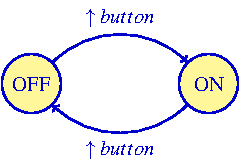
\includegraphics[width=0.30\columnwidth]{./Unit-01/img/DynSys-LampAutomaton.pdf}
       \end{center}
 \item In our activity we are not addressing this kind of systems.
 \item Let us move to a \emph{rough} (system class)--(control problem) pairing.
 \end{itemize}
\end{frame}

\begin{frame}
\frametitleTC{Dynamic systems classes and control problems}
\framesubtitleTC{...this time looking at computers -- just an overview to stimulate discussion}
\myPause
 \begin{itemize}[<+-| alert@+>]
 \item Group 1 -- problems directly related to physics \emph{stricto sensu}:
       \begin{itemize}[<+-| alert@+>]
       \item typical example -- CPU temperature;
       \item system model -- continuous-time dynamic system;
       \item controller design -- as continuous-time system, then converted to discrete-time\\
             to become control \TC{code}.
       \end{itemize}
 \item Group 2 -- problems not in group 1 where requirements are translatable into desired behaviours
       of signals (reference or admissible range):
       \begin{itemize}[<+-| alert@+>]
       \item typical example -- deadline enforcement, obtained by tracking a desired completion\\
             that reaches 100\% by the deadline (\underline{many} problems can be formulated\\
             this way or analogously);
       \item system model -- discrete-time dynamic system;
       \item controller design -- as discrete-time system, then code.
       \end{itemize}
 \item Group 3 -- anything else:
       \begin{itemize}[<+-| alert@+>]
       \item mixed design strategy (not in the scope of our activity),
       \item or not suited for a control-theoretical design.
       \end{itemize}
 \end{itemize}
\end{frame}

